\documentclass{beamer}

\usepackage{mystyle}

\usepackage{Sweave}
\begin{document}
\Sconcordance{concordance:documento.tex:documento.Rnw:%
1 3 1 1 0 8 1}
\Sconcordance{concordance:documento.tex:./tex/intro.Rnw:ofs 13:%
1}
\Sconcordance{concordance:documento.tex:documento.Rnw:ofs 14:%
14 2 1}


\title{Demo Meraki}
\titlegraphic{
\includegraphics[width=4cm]{img/isat.jpg}}
\author{Manuel}

\frame{\titlepage}

\section{\hspace{1in}Meraki}
\begin{frame}
\frametitle{\currentname}
\begin{figure}[H]

\includegraphics[width=4cm]{img/meraki.png}
\end{figure}
\emph{Cisco Meraki} es un conjunto de herramientas que permiten la unificación de la administración de la red sobre ubicaciones, infraestructuras y dispositivos. \\ 
Entre sus componentes se incluyen:
\begin{enumerate}
\item Solución completa de administración de la red desde la nube.
\item Administración de Wireless, Switching, Seguridad y SD-WAN, Administración de Dispositivos Móviles (MDM), y Cámaras Inteligentes.
\item Hardware, software y servicios en la nube integrados entre sí.
\end{enumerate}
\end{frame}

\subsection{\hspace{1in}Integraciones Meraki}
\begin{frame}
\frametitle{\currentname}
Existen 5 vías mediante las cuales una aplicación puede extender las funcionalidades de Meraki.
\begin{enumerate}
\item \emph{Dashboard API} \\
Servicio RESTful de suministro, administración y monitoreo de dispositivos.
\item \emph{WebHook Alerts} \\
Notificaciones en tiempo real de la salud de la red
\item \emph{Location Scanning API} \\
Método HTTP POST que envía posiciones (GPS, X/Y) basado en APs Meraki
\item \emph{MV Sense} \\
Vistas en tiempo real de imagen y posición desde cámaras MV
\item \emph{External Captive Portal (EXCAP)} \\
Uso de la red WiFi para construir lealtad del cliente
\end{enumerate}
\end{frame}

\section{\hspace{1in}Meraki Scanning API}
\begin{frame}
\frametitle{\currentname}
La Meraki Scanning API\footnote{Una API es una interfaz mediante la cual se comunican 2 programas de computadora} hace solicitudes que deben de ser atendidas por un servidor web.
\begin{figure}[H]
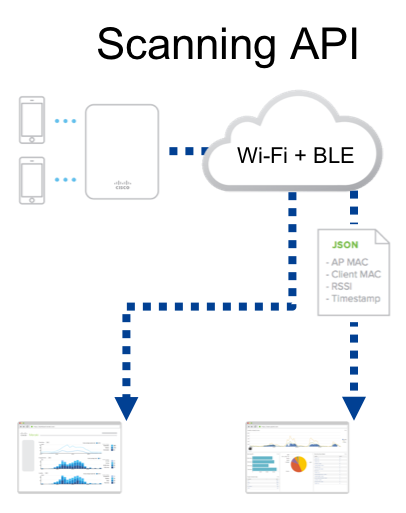
\includegraphics[width=4cm]{img/scanningapi.png}
\end{figure}
\end{frame}

\subsection{\hspace{1in}Arquitectura}
\begin{frame}
\frametitle{\currentname}
El flujo de la información es muy sencillo. Cada uno de los APs envía al Dashboard de Meraki una estimación de la distancia a la que se encuentran los dispositivos (WiFi y BLE). En un servicio en la nube esta información se procesa para dar un estimado de la posición (GPS/XY) de cada dispositivo y se envían en formato JSON mediante POSTs HTTP que han de ser recibidor por un servidor identificado por el Dashboard.
\begin{figure}[H]
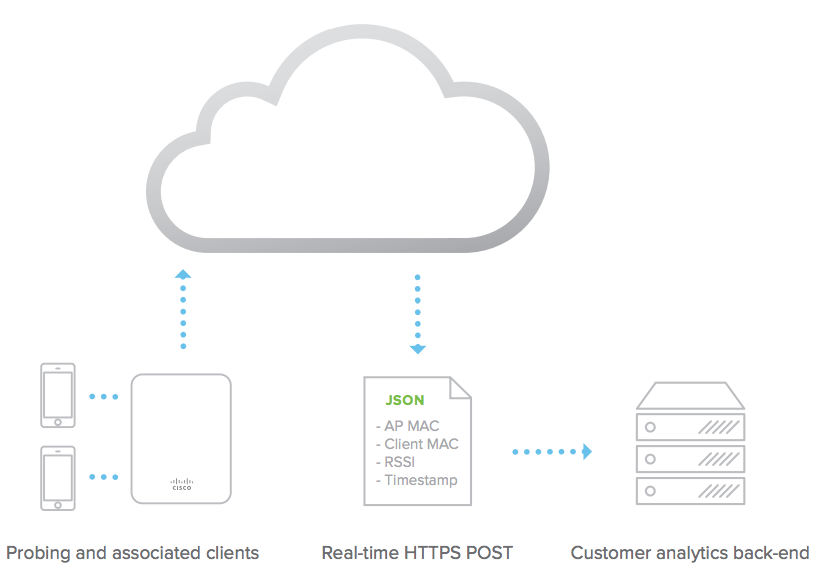
\includegraphics[width=4cm]{img/merakiarq.png}
\end{figure}
\end{frame}

\section{\hspace{1in}Casos posibles de uso}
\begin{frame}
\frametitle{\currentname}
Registro de visitas o asistencias
\begin{figure}[H]
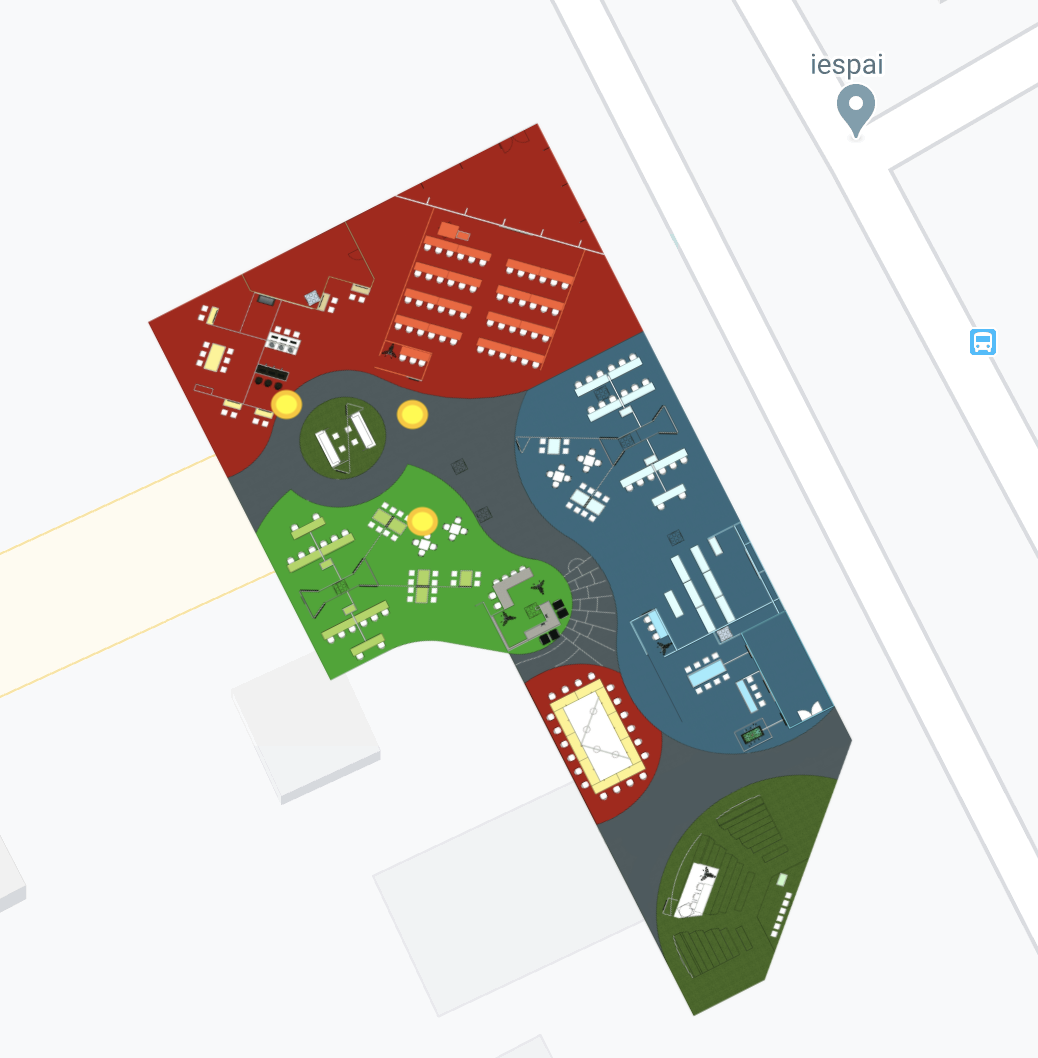
\includegraphics[width=4cm]{img/posiciones.png}
\end{figure}
\end{frame}

\begin{frame}
\frametitle{\currentname}
Rastreo y seguimiento de equipos o materiales valiosos
\begin{figure}[H]
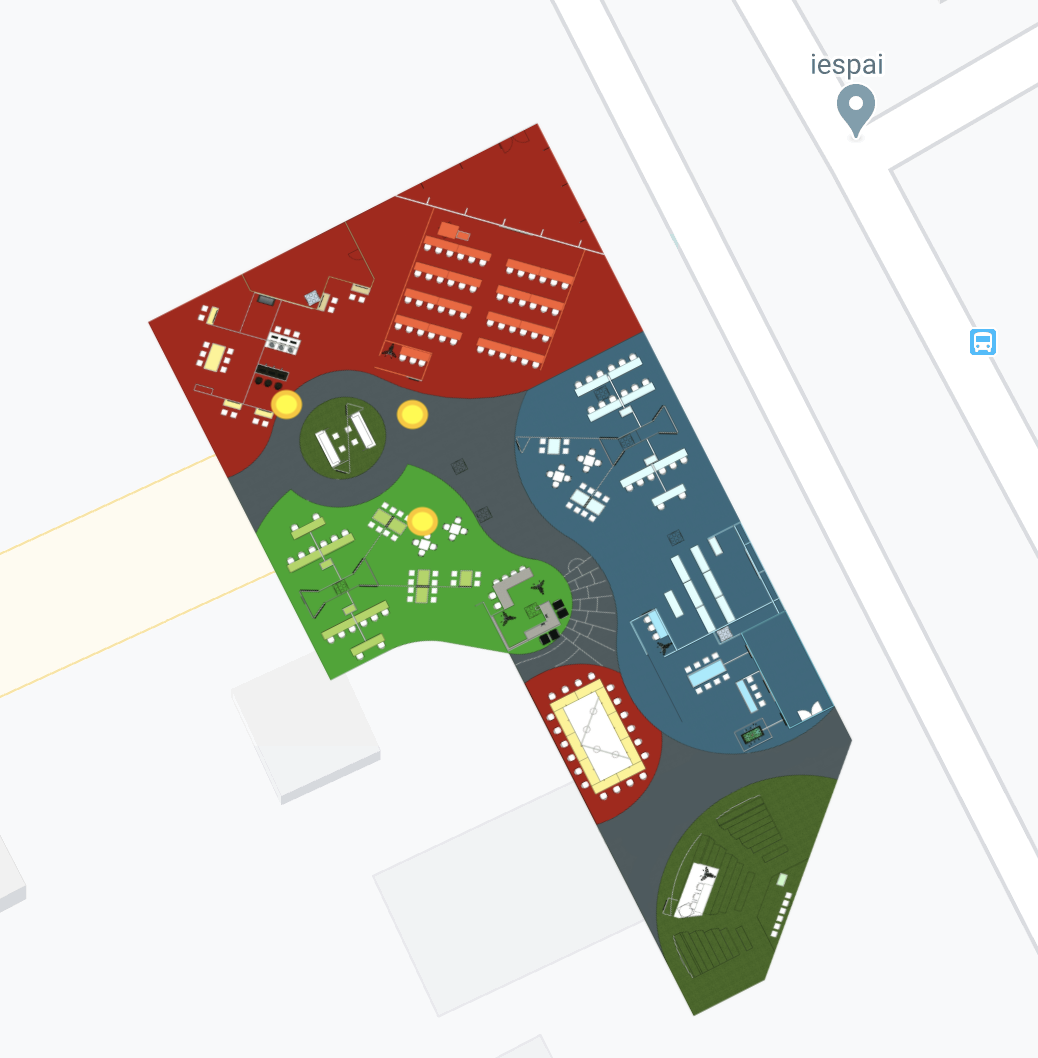
\includegraphics[width=4cm]{img/posiciones.png}
\end{figure}
\end{frame}

\begin{frame}
\frametitle{\currentname}
Conteo de visitas a áreas específicas dentro del alcance de los APs Meraki
\begin{figure}[H]
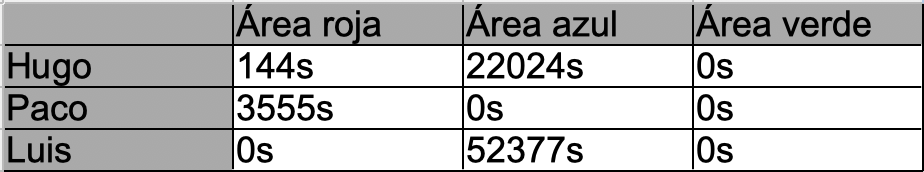
\includegraphics[width=4cm]{img/tablapos.png}
\end{figure}
\end{frame}

\begin{frame}
\frametitle{\currentname}
Medición de la distancia entre dispositivos móviles
\begin{figure}[H]
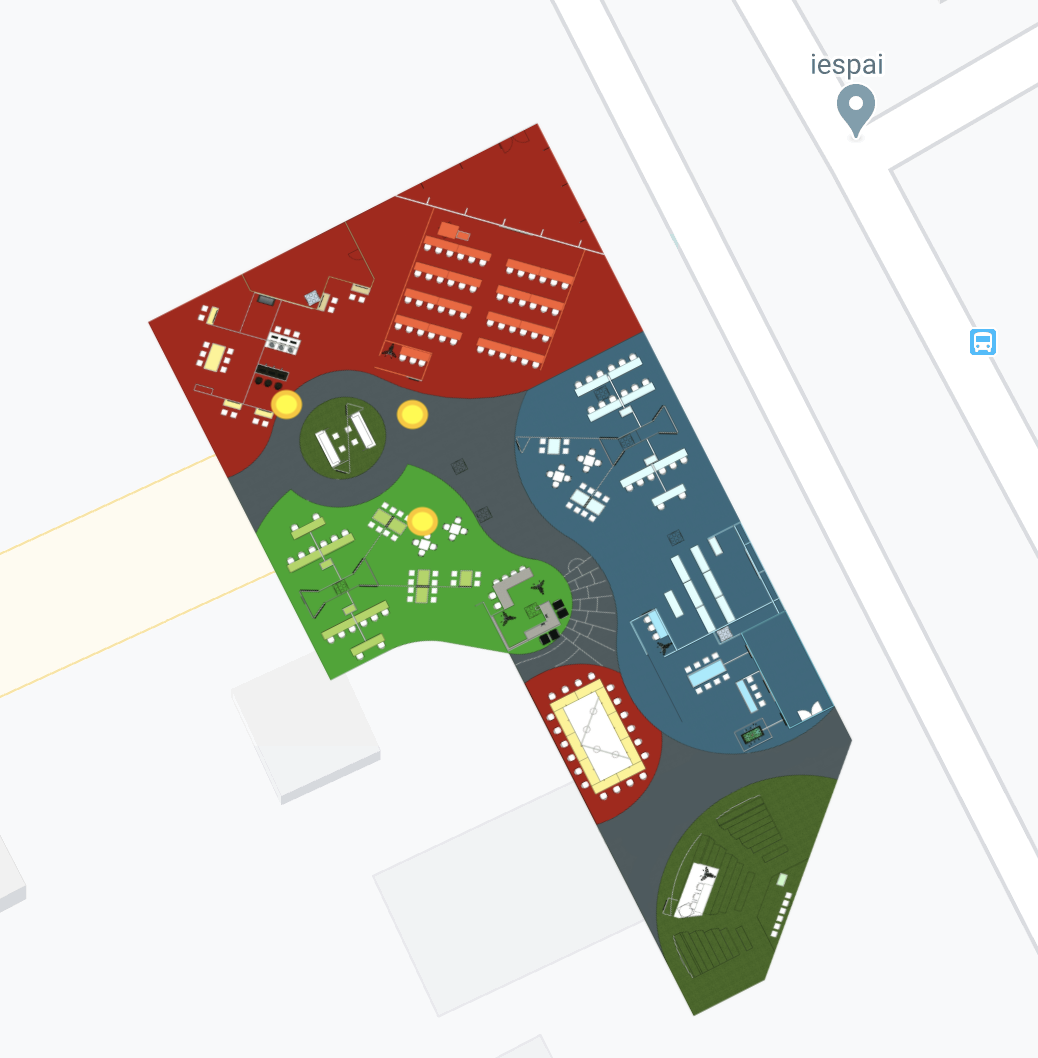
\includegraphics[width=4cm]{img/posiciones.png}
\end{figure}
\end{frame}

\begin{frame}
\frametitle{\currentname}
Identificación, almacenamiento y posterior análisis de la ruta que siguió un dispositivo móvil.
\end{frame}

\begin{frame}
\frametitle{\currentname}
Identificación de grupos de dispositivos
\end{frame}

\end{document}
